\chapter{Background and Theory}
This chapter will introduce the reader to the necessary information needed to understand the background and theoretical motivations that underpin this thesis. In Section \ref{ML}, the reader will be introduced to the basic concepts required to understand this thesis. The theory mainly involves the terminology and the methodology of training and evaluating machine learning models with a focus on deep neural networks. A reader who is well versed in these areas can skip this section. Section \ref{metalearning} will explain the concepts of meta-learning and few-shot learning and introduce the reader to the \gls{MAML} algorithm and its underlying theory. Section \ref{previous-work} will cover previous research related to synthetic data generation. Section \ref{related-work} will cover some examples of contemporary work that have attempted to solve similar issues related to meta-learning as this thesis. Section \ref{approach} will, in detail, outline the proposed approach. It will also outline the advantages of the suggested approach in comparison to existing methods.

\section{Machine Learning}\label{ML}
Machine learning is a field of study concerned with creating models that learn by utilizing statistics extracted from previously observed data. There are several forms of learning algorithms. \textit{supervised learning} refers to training a model on a set of labelled training data $\mathcal{D} = \{\bm{X}, \bm{Y}\}$ where $\bm{X} = \{\bm{x}_1, \dots, \bm{x}_n\}$ are the input data and $\bm{Y} = \{y_1, \dots, y_n\}$ are \textit{labels} that define the output of the function $F: \mathbb{R}^n \to \mathbb{R}$ the algorithm should learn. The learning is supervised in the sense that the algorithm can inspect the label $y_i$ of each datum $x_i$ to asses how well it performs. This assessment is commonly done by computing a cost (or loss) function, which assesses the disparity between the algorithms guess $\hat{y}_i$, and the true label $y_i$~\cite{deeplearningbook}.

In contrast, \textit{unsupervised learning} refers to the problem of training an algorithm on unlabeled training data. This lack of labeling forces the algorithm to learn and infer properties of the data on its own, without the aid of a supervisor~\cite{deeplearningbook}.

\subsection{Generalization and Overfitting}
The goal of any machine learning algorithm is to be able to generalize well to previously unseen data. Generalization as a concept can be formally defined as the error rate the model or algorithm exhibits on unseen data. A lower error on this test-data implies higher generalization and vice versa~\cite{deeplearningbook}.

Every machine learning model possesses two attributes that relate to its ability to generalize. One is \textit{bias}, expressed as $E[\hat{f}(x) - f(x)]$, which is the difference between the expected prediction of the model and the true value it tries to predict. A model with high bias will \textit{underfit} to the training data, resulting in high training error rates. The reason why is because high bias models are inherently limited in what they can learn, and are restricted to a more narrow problem domain then what the training task requires~\cite{bishop}. 

The other is \textit{variance}, which refers to the expected squared difference between each prediction and the average prediction: $E\Big[(\hat{f}(x) - E[\hat{f}(x)])^2\Big]$. For a model with high variance, small changes in the training data can strongly affect the predictions on the test data. Such a model is sensitive to noise and random patterns in the training data. As a result, it will often \textit{overfit} to training data, showing low error rates during training, while generalizing poorly on the test data~\cite{bishop, deeplearningbook}.

The \textit{bias-variance trade off} is a fundamental concept within machine learning which refers to the relationship between the \textit{bias} and the \textit{variance}. Reducing the variance of a model will invariably result in an increase in its bias, and vice versa. To optimize performance in a model, one needs to find a proper balance between bias and variance. Finding a proper balance can, for example, be done by \textit{regularization}, which entails adding certain restrictions to a high-variance model in order to lower its variance~\cite{bishop}.

\subsection{Deep Learning}
Deep learning is a subfield within machine learning that focuses on the study of \glspl{ANN} and deep architectures. The field has, in recent years, seen a substantial increase in popularity, despite the technology dating back to the 1980s, with the \gls{MLP} and the back-propagation algorithm. Large public datasets, increasingly powerful hardware, as well as increased knowledge of how these models can be trained, have all contributed to its recent rise to popularity~\cite{deeplearningbook}.

%\begin{equation} o =\sum_i(w_i x_i) + b \end{equation}
\tikzset{basic/.style={text width=1em,text badly centered}}
\tikzset{input/.style={basic}}
\tikzset{weights/.style={basic}}
\tikzset{functions/.style={draw, basic,circle}}

\begin{figure}
    \centering
    \begin{tikzpicture}
        \node[functions] (center) {$\alpha$};
        \node[right of=center] (right) {};
            \path[draw,->] (center) -- (right);
        \node[functions,left=3em of center] (left) {$\sum$};
            \path[draw,->] (left) -- (center);
        \node[weights,left=3em of left] (2) {$w_2$} -- (2) node[input,left of=2] (l2) {$x_2$};
        
        
        \node[above=3em of left] (bias) {$b$};
            \path[draw,->] (bias) -- (left);
        
            \path[draw,->] (l2) -- (2);
            \path[draw,->] (2) -- (left);
        \node[below of=2] (dots) {$\vdots$} -- (dots) node[left of=dots] (ldots) {$\vdots$};
        \node[weights,below of=dots] (n) {$w_n$} -- (n) node[input,left of=n] (ln) {$x_n$};
            \path[draw,->] (ln) -- (n);
            \path[draw,->] (n) -- (left);
        
        \node[weights,above of=2] (1) {$w_1$} -- (1) node[input,left of=1] (l1) {$x_1$};
            \path[draw,->] (l1) -- (1);
            \path[draw,->] (1) -- (left);
        \node[weights,above of=1] (0) {$w_0$} -- (0) node[input,left of=0] (l0) {$1$};
            \path[draw,->] (l0) -- (0);
            \path[draw,->] (0) -- (left);
            
    \end{tikzpicture}
    \caption{Single neuron with $n$ inputs and activation function $\alpha$}
    \label{fig:neuron}
\end{figure}

The core of an \gls{ANN} is a basic linear unit called a \textit{neuron}, \textit{node} or \textit{perceptron} (see Figure \ref{fig:neuron}), which is superficially inspired by the neurons in the human brain. These neurons compute the weighted sum of the input vector $\mathbf{x}$ with added an offset called \textit{bias} ($\beta$ in Figure \ref{fig:neuron}). A non-linear activation function is then applied to the output of the neuron ($\alpha$ in Figure \ref{fig:neuron}). The activation function allows the network to express more complex functions than strictly linear ones. This activation function can be any non-linear differentiable function, but the most common function is the \gls{RELU}~\cite{deeplearningbook}.

A set of parallel neurons that are joined together make up a layer. An \gls{ANN} is constructed by stacking several of these layers, by letting the output of one layer become the input to the next layer (see Figure \ref{fig:ann}). The network then takes some input vector $x$, feeds it through each layer in the network, and lets the final layer, the output layer, produce the network's prediction $\hat{y}$. If the task is a classification task, a \textit{softmax} function is often applied to the final prediction vector $\hat{y}$. The softmax function normalizes the values in the vector to a valid probability distribution~\cite{deeplearningbook}.

\def\layersep{3cm}
\begin{figure}[h]
\centering
\begin{tikzpicture}[shorten >=1pt,->,draw=black, node distance=\layersep]
    \tikzstyle{every pin edge}=[<-,shorten <=1pt]
    \tikzstyle{neuron}=[circle,fill=white!25,minimum size=17pt,inner sep=0pt]
    \tikzstyle{input neuron}=[neuron, draw=black, thick];
    \tikzstyle{output neuron}=[neuron, draw=black, thick];
    \tikzstyle{hidden neuron}=[neuron, draw=black, thick];
    \tikzstyle{annot} = [text width=4em, text centered]

    % Draw the input layer nodes
    \foreach \name / \y in {1,...,4}
    % This is the same as writing \foreach \name / \y in {1/1,2/2,3/3,4/4}
        \node[input neuron, pin=left:$x^{1}_\y$] (I-\name) at (0,-\y) {};

    % Draw the hidden layer nodes
    \foreach \name / \y in {1,...,5}
        \path[yshift=0.5cm]
            node[hidden neuron] (H-\name) at (\layersep,-\y cm) {};

    % Draw the output layer node
    \node[output neuron,pin={[pin edge={->}]right:$\hat{y}_1$}, right of=H-3] (O) {};

    % Connect every node in the input layer with every node in the
    % hidden layer.
    \foreach \source in {1,...,4}
        \foreach \dest in {1,...,5}
            \path (I-\source) edge (H-\dest);

    % Connect every node in the hidden layer with the output layer
    \foreach \source in {1,...,5}
        \path (H-\source) edge (O);

    % Annotate the layers
    \node[annot,above of=H-1, node distance=1cm] (hl) {Hidden layer};
    \node[annot,left of=hl] {Input};
    \node[annot,right of=hl] {Output};
\end{tikzpicture}
\caption{Simple ANN with a single hidden layer.}
\label{fig:ann}
\end{figure}

\subsection{Convolutional Neural Networks}
The \gls{CNN} is a specific form of neural network that is specialized in processing grid-like input maps, such as images. A standard \gls{CNN} consists of a set of stacked \textit{convolutional layers}, followed by a set of \textit{fully-connected} layers, similar to a standard neural network. The main building block, the \textit{convolutional layer}, consists of three main components: A set of \textit{kernels}, an non-linear \textit{activation function} and a resolution reducing \textit{pooling layer}~\cite{deeplearningbook}.

The \textit{kernels} (or \textit{filters}) consist of a set of trainable weights that, similarly to the perceptron, apply a linear function to regions in the grid-like input. These regions, also known as receptive fields, are laid out in a grid-like fashion over the input, in order to preserve the input's spatial information. The resulting grid-like output of a kernel is commonly referred to as a \textit{feature-map}. A single layer commonly has a large number of kernels, which each learns to identify some feature in the input~\cite{deeplearningbook}.

The \textit{activation function} is a non-linear function, such as \gls{RELU}, that is applied to the feature-maps outputted by the kernels. Similarly to its use in ANNs, it serves the purpose of allowing the networks to express more complex, non-linear functions. Similarly to ANNs, a common choice for activation function is the \gls{RELU}~\cite{deeplearningbook}.

The \textit{a pooling layer} applies a pooling operator, such as \textit{max} or \textit{mean}, over regions in the feature maps (see Figure \ref{fig:pool}). The pooling layer reduces the overall resolution of the outputted feature maps, while still retaining the essential information. Reducing the dimensionality of the output have the advantage of requiring less trainable weights in later layers, reducing the risk of overfitting~\cite{deeplearningbook}.

\begin{figure}[H]
    \centering
    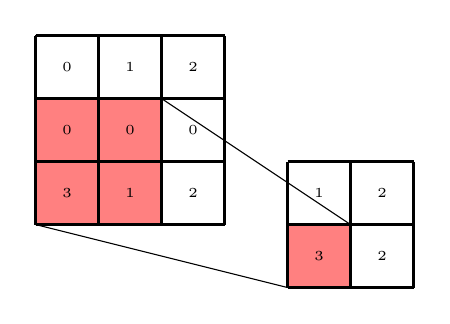
\begin{tikzpicture}[scale=0.8,every node/.style={minimum size=1cm}]
            \draw[fill=white] (-4,0) rectangle (-1,3);            
            \draw[fill=red!50] (-4,0) rectangle (-2,2);
            \draw[draw=black,thick] (-4,0) grid  (-1,3);    
                           
            
            \node (000) at (-3.5,2.5) {\tiny 0};
            \node (001) at (-2.5,2.5) {\tiny 1};
            \node (002) at (-1.5,2.5) {\tiny 2};
            
            \node (010) at (-3.5,1.5) {\tiny 0};
            \node (011) at (-2.5,1.5) {\tiny 0};
            \node (012) at (-1.5,1.5) {\tiny 0};
            
            \node (020) at (-3.5,0.5) {\tiny 3};
            \node (021) at (-2.5,0.5) {\tiny 1};
            \node (022) at (-1.5,0.5) {\tiny 2};
         
         
             
             \draw[fill=white] (0,-1) rectangle (2,0);
            \draw[fill=red!50] (0,-1) rectangle (1,0);            
            \draw[draw=black,thick] (0,-1) grid (2,1);

             \draw (-4,0) -- (0,-1);
             \draw (-2,2) -- (1,0);
                 
            \node (100) at (0.5,0.5) {\tiny 1};
            \node (101) at (1.5,0.5) {\tiny 2};

            \node (110) at (0.5,-0.5) {\tiny 3};
            \node (111) at (1.5,-0.5) {\tiny 2};            
    \end{tikzpicture}
    \caption{Example of Max Pooling}
    \label{fig:pool}
\end{figure}

Some convolutional layers also include an additional component called a \textit{batch-normalization layer}. The batch-normalization layer is a function that scales its input to have zero mean and unit variance, with respect to all inputs in the current mini-batch. This function is most commonly applied before the activation function to make the network learn faster~\cite{batchnorm}.

\subsection{Training Neural Networks}
Feed forward neural networks are trained in a \textit{supervised fashion} where it is presented with data-and-label pairs $(x_i, y_i)$, and aims to minimize a task-specific loss or cost function $\mathcal{L} \rightarrow \mathbb{R}$. This loss function is a measurement of the disparity of the network's guess $f_{\theta}(x_i) \rightarrow \hat{y}_i$ and the ground truth value $y_i$.

The networks are trained using an iterative optimization algorithm, called \textit{gradient descent}. At each iteration, the algorithm computes the gradient of the network using the training data and moves the weights one step proportional to the negative gradient. Moving along the negative gradient can be conceptualized as trying to go down a hill, and at every step walking down the direction which has the steepest slope~\cite{deeplearningbook}.

More formally, if some network is parameterized by $w_t$ at iteration $t$ and the goal is to minimize loss function $L$ then a single step of gradient descent is expressed as:

\begin{equation}
    w_{t+1} = w_{t} - \alpha \partder{L}{w_t}
\end{equation}

Where the \textit{learning rate} $\alpha$ is a \textit{hyperparameter}, a variable that needs to be manually set before training the network. The learning rate defines how big of a step the parameters should move in each iteration. If $\alpha$ is too high, the algorithm will move erratically, often overshooting good local minima. On the other hand, if the learning rate is too low, the algorithm will take too long to converge~\cite{deeplearningbook}.

There exist a set of different versions of gradient descent, each with different approaches to getting an estimate of the current gradient. In \textit{batch gradient descent} the gradient is computed over all the training examples in the training set. Using all data points provides an unbiased estimate of the gradient, but is often computationally expensive to calculate. \textit{Stochastic gradient descent} instead samples a random data point from the training set at each iteration, and uses that single data-point to compute the gradient estimate. This estimate is often noisier than the batch approach but is significantly faster to compute. Lastly, \textit{mini-batch gradient descent} is a combination of the two previous methods. It randomly samples a small \textit{mini-batch} of examples at each update, and uses that mini-batch to compute a less noisy estimate of the gradient estimate~\cite{deeplearningbook}.

The solution space of neural networks is both non-linear and non-convex. Therefore, gradient descent is not guaranteed to reach the global minimum of the loss-function, since the negative gradient can be pointing towards local minima. To counteract this, there exists modifications to the gradient descent algorithms that attempt to use previous knowledge of the solution space to guide the network towards better solutions~\cite{deeplearningbook}. One example of such an algorithm is the \textit{momentum} algorithm, which stores an exponential moving average over all previous gradients. This average is then used as the update direction, rather than the standalone gradient. More formally, the update for a single weight $w_t$ at time $t$ with momentum becomes:

\begin{equation}w_{t+1} = w_{t} - \alpha V_t\end{equation}
where 
\begin{equation}V_t = \beta V_{t-1} + (1-\beta)\partder{L}{w_t}\end{equation}
Here, $\alpha$ is the normal learning rate, and $\beta$ is a manually set hyper-parameter that determines how quickly the old gradients should be forgotten.

Another optimization algorithm is the \textit{Adam} algorithm. In addition to keeping a moving average over past gradients, this algorithm also uses an adaptive learning rate for each individual weight. These adaptive learning rates are calculated using a exponential moving average over past square gradients. More formally, the update for a single weight $w_t$ at time $t$ becomes:

\begin{equation}w_{t+1} = w_t - \frac{\alpha}{\sqrt{\hat{S}_t + \epsilon}} \hat{V}_t\end{equation}
where 
\begin{equation}\hat{V}_t = \frac{V_t}{1-\beta^t_1}\end{equation}
\begin{equation}\hat{S}_t = \frac{S_t}{1 - \beta^t_2}\end{equation}

\begin{equation}V_t = \beta_1 V_{t-1} + (1-\beta_1)\partder{L}{w_t}\end{equation}
\begin{equation}S_t = \beta_2 S_{t-1} + (1 - \beta_2)\left(\partder{L}{w_t}\right)^2\end{equation}

Here, $\alpha$ is the base learning rate, $\epsilon$ is a small value that prevents division by zero, and $\beta_1$ and $\beta_2$ adjust the two moving averages.


\subsection{Data Augmentation}\label{augmentation}
Data augmentation is a common approach to artificially increase training data by applying label invariant transforms to existing data. These transformations are commonly known as augmentation functions. Data augmentation is a standard way in deep learning to reduce overfitting when the amount of actual data is scarce. It can also have the added effect of introducing noise in the training process, which can also help prevent overfitting~\cite{deeplearningbook}.

The choice of augmentation function is highly domain-specific since the transforms that are label invariant varies between domains. For example, rotating an image of a dog 180 degrees does not change its natural class, it still portrays a dog. However, rotating an image containing the digit nine 180 degrees would change its class from nine to six. 

Generally, if one has a set of classes $C_0,...C_{m-1}$ and a set of data points $x_0,...,x_{n-1}$ and an augmentation-function $A$, then one wants $x_i \in C_j, A(x_i) \in C_j$ to hold for the augmentation function~\cite{deeplearningbook}.

Standard augmentation functions for image data include: flipping images horizontally/vertically, rotating images, adding random image noise, and adjusting contrast and saturation~\cite{deeplearningbook}.

\subsection{Transfer Learning}
Transfer learning is a field within machine learning that focuses on utilizing knowledge gained while solving one problem and applying it to a related but different problem. The idea is that for two related tasks, a \textit{source task} and a \textit{target task} there exist an overlap of knowledge that can be extracted from the source task and used to aid in the learning of the target tasks. For example, a person that learns to play the piano will have an easier time to learn playing guitar later, compared to a person who has no prior musical experience. The reason is that there is an overlap in terms of knowledge between the \textit{source task} of learning piano, and the target task of learning guitar, for example reading sheet music, a sense of rhythm and finger dexterity. Transfer learning aims to apply the same logic to machine learning tasks~\cite{transferlearning}.   

A common approach to transfer learning is to extract the first set of layers of a \gls{CNN} trained on a large amount of labeled data, such as the ImageNet dataset~\cite{imagenet}. These first layers output a set of generic mid-level features that are useful for a variety of visual tasks~\cite{cnn-features}. To correct for any difference in distribution between the source and the target domain, a set of additional adaption layers are appended to these extracted layers. These adaption layers are then trained on a small set of labeled data from the target domain, while the previously extracted layers remain locked in place. This approach is called \gls{TCNN} and is one of the most common methods when training deep \gls{CNN}s~\cite{transferlearning}.

\subsection{Multi-Task Learning/Joint Learning}\label{MTL}
Joint Learning or \gls{MTL} is a method of training models that aims to improve the model's ability to generalize by forcing it to learn multiple tasks simultaneously. The model is trained on several distinct but domain-related tasks and aims to reduce the expected cost over all the tasks. The intuition behind this approach is that by forcing a network to learn to use the same input data for different tasks, the network will be forced to have a more general internal feature representation that will prevent overfitting and improve overall performance ~\cite{multi-task-learning}. 

\gls{MTL} for neural networks is done using either \textit{soft} or \textit{hard parameter sharing} of the hidden layers. In hard sharing, the initially hidden layers of the network are shared between all tasks, while each task has a unique set of final output layers. In soft sharing, each task has a unique network, but the difference between the weights in the networks are regularized on a layer by layer basis in order to force the networks to be more similar~\cite{multi-task-learning}.

\section{Few-Shot Learning and Meta-Learning}\label{metalearning}
Few-shot learning is a specific form of machine learning problem, where limits are set on how much data a model is allowed to observe during training. For most machine learning and deep learning tasks, the model is provided an extensive training set from which to learn. In contrast, in few-shot learning tasks, the models are only provided a handful of examples during training, with the number of examples being an integral part of the problem definition~\cite{maml}. 

For classification problems it is common to use the description $N$-way $K$-shot learning, where there are \textit{N} distinct classes and the model is allowed to train using \textit{K} examples from each class. $K$ should be small in order for the task to be considered a few-shot learning tasks. For regression, it is instead common to use the term $K$-shot learning, where $K$ is the total number of data points the model is allowed to observe~\cite{maml}.

%\subsection{Meta-Learning}
Meta-learning, or learning how to learn, is a concept within machine learning that has its origin in the late 1980s~\cite{unsup-maml-rand}. Although the term has been applied to various scenarios throughout the literature, meta-learning generally refers to a training scenario in which a model learns on two different levels. An initial \textit{meta-learning phase} where the model gradually acquires knowledge across various tasks $T_1, ..., T_N$, and a second \textit{meta-testing phase} where the previously meta-trained model is trained on previously unseen tasks $T_{N+1}$ with a limited number of examples~\cite{maml, unsup-maml-rand, santoro}. 

\change{Meta-learning is a common method for tackling few-shot learning problems. The idea is that by having a model meta-train on few-shot learning task, the model can then learn a method of learning, allowing it to quickly learn previously unseen few-shot tasks. 
%A \textit{task} is a very general concept that can be difficult to properly define, but can consist of everything from different forms of classification to reinforcement problems. In its most general form a task can be considered a mapping from some observation $x$ to some output $\textbf{a}$. More formally this can be expressed as
%$T=\{\mathcal{L}(x_1, \textbf{a}_1,...,x_{H}, \textbf{a}_H), q(x_1), q(x_{t+1}|x_t, \textbf{a}_t), H\}$. 
%Here, $q(x_t)$ is the distribution over initial observations. $q(x_{t+1}|x_t, \textbf{a}_t)$ is the transition distribution between observations. $H$ is the number of episodes, which for independently and identically distributed samples is 1. Lastly, $\mathcal{L} \rightarrow R$ is the task-specific loss function used to guide the learning process when it trains using gradient descent.

In order to sample few-shot classification tasks, one needs a large dataset with a large set of classes. As an example, one can consider the Omniglot dataset~\cite{omniglot}. It consists of 1623 different characters from a range of different alphabets, with each character having twenty hand-drawn examples. Sampling 5-way 1-shot classification tasks from this dataset would entail randomly selecting five classes from the complete set of 1623 and taking one example from each class as training data.}

There are many different approaches to meta-learning. One example is memory-augmented neural networks~\cite{santoro}. These recurrent networks have access to an external memory module to which it can read and write freely. The external memory module allows it to quickly encode new information, which in turn makes it very suitable to learn new tasks quickly. 

Another example is meta-networks~\cite{meta-networks}. These networks relies on a concept called \textit{fast} and \textit{slow} weights. The slow weights are updated using normal gradient descent. The fast weights, however, are updated by an external meta-learner module that uses input from both the original model, as well as knowledge of previous tasks, to predict the new weights. The fast and slow weights are then combined in the final prediction~\cite{meta-networks}.

Another approach to meta-learning is \textit{metric learning}. Rather than training a model to learn new tasks, metric learning aims to find a task-invariant similarity metric across the set of training tasks~\cite{siamese}. This metric can then be used classify an entirely new set of classes by comparing the test samples to the labeled training samples. A few examples of these approaches are the Siamese Neural Networks~\cite{siamese} and the Matching Network~\cite{matching}.

\glsreset{MAML} \change{Removed section}
The meta-learning method used in this thesis is \gls{MAML}~\cite{maml}. Unlike most other methods it does not require any specialized model architecture and can be used with any gradient descent trained model. The goal of \gls{MAML} is to find a weight initialization that is optimized for learning new tasks. Finding such a weight initialization can be conceptualized as finding an internal feature representation that generalizes to a broad range of tasks~\cite{maml}. With such a representation, the top-layers of, e.g., a neural network can be fine-tuned to a new task in a couple of gradient steps~\cite{maml}.

\begin{algorithm}[H]
\SetAlgoLined
\SetKwInOut{Input}{Input}
\SetKwInOut{Output}{Output}
\Input{$p(T)$: distribution over tasks}
\Input{$\alpha, \beta$: step size parameters}
Randomly initialize $\bm{\theta}$ \\
\While{\text{not done}} {
    Sample meta-batch of tasks $T_1,...,T_n \sim p(T)$ \\
    where each task $T_i$ contains training data $\mathbf{x}_i$ and validation data $\mathbf{x}'_i$\\
    \ForEach{$T_i$} {
        Update: $\theta_i'  \leftarrow \theta - \alpha \nabla_{\theta} \mathcal{L}_{T_i}(f_{\theta}^{\mathbf{x}_i})$
    }
    Update $\theta \leftarrow \theta - \beta \nabla_{\theta}\sum^{n}_{i=1} \mathcal{L}_{T_i}(f_{\theta'_i}^{\mathbf{x}'_i})$
}
\bo{return } $\theta$ 
\caption{Model-Agnostic Meta-Learning}
\label{alg:maml}
\end{algorithm}

\gls{MAML} is outlined in Algorithm \ref{alg:maml}. Input to \gls{MAML} consist of a distribution over tasks $p(T)$ and a model $f_{\theta}$ parameterized by $\theta$. It also uses two additional hyperparameters: $\alpha$, the learning rate for the inner update step and $\beta$, the learning rate for the outer update step.

During training, a fixed number of tasks $T_i$ are sampled for each meta iterations. The sampled tasks are referred to as a \textit{meta-batch}, and the number of tasks to be sampled during each step is referred to as the \textit{meta-batch size}. 

Each training step in \gls{MAML} is divided into two distinct steps: First, an inner, task-specific update step called the \textit{inner update step}. Second, an outer meta-training step called the \textit{outer update step}. For each task $T_i$ in a meta-batch, a training set $\mathbf{x}_i$ and a validation set $\mathbf{x}'_i$ is sampled. The training set $\mathbf{x}_i$ is used during the inner update step, while the validation set $\mathbf{x}'_i$ is used during the outer update step.

In the inner update step, the the current model parameters $\theta$ are updated using batch gradient descent with the sampled task-specific training data $\mathbf{x}_{i}$ and the task-specific loss $\mathcal{L}_{T_i}$. (To keep the notation simple the number of update steps are limited to 1, but in practice it can be extended to any number of steps.) This update step results in the updated parameters $\mathbf{\theta}'_{i} = \theta- \alpha\nabla_{\theta}\mathcal{L}_{T_i}\left(f_{\theta}^{\mathbf{x}_{i}}\right)$ for each task $T_i$ in the meta-batch. 

In the outer update step, the task-specific loss $\mathcal{L}_{T_i}$ is computed with the task-specific validation data $\mathbf{x}'_{i}$ and the task-specific parameter $\theta_i$ from the inner update step. These losses of all the tasks in the meta-batch are then added together, serving as a measurement on how well $f_{\theta}$ was able to learn the tasks. 

The training objective of \gls{MAML} can be formalized as:
\begin{equation} \min_{\theta} \sum_{T_i \sim p(T)} \mathcal{L}_{T_i}\left(f_{\theta'_i}^{\mathbf{x}'_{i}}\right)\end{equation}

This objective can be interpreted as finding a parameter setting $\theta$ that minimizes the expected loss after the inner update step on all the tasks sampled from the task distribution. Such a parameter setting $\theta$ would mean the model was in a good position to quickly learn a new task. \gls{MAML} uses gradient descent to optimize for this objective, computing the gradient with respect to $\theta$ over the current meta-batch. In practice, a more sophisticated gradient method can also be used, like for example Adam.

\change{Removed a section header}
%\subsubsection{First-Order MAML and Reptile}\label{fomaml}
The outer update step in the \gls{MAML} algorithm requires computing the gradient through a gradient update, which requires the computation of the second ordered Hessian Matrix. Computing the Hessian matrix for a neural network can be computationally expensive and can increase training time significantly. In order to speed up learning it is possible to ignore the second order gradients by considering parameters $\theta'_i$ as constant during the outer update.~\textcite{maml} showed that although this has a slightly negative effect on performance, it will still produce result comparable to the standard \gls{MAML} method. This first-order modification of the \gls{MAML} algorithm is called \gls{FOMAML}.

A modification to the \gls{FOMAML} algorithm called Reptile was later proposed by \textcite{reptile}. Similarly to \gls{FOMAML}, Reptile does not compute the second order gradients of the outer update. However, Reptile takes this one step further by completely ignoring the use of validation data. Instead, it uses the averages of the task-specific weight update $\theta'_i$ to compute the outer update step. 

This approach makes the training more akin to \gls{MTL} (see Section \ref{MTL}) than \gls{MAML}, at least when performing a single update step during training. Averaging over $\theta'_i$  also makes it easier for Reptile to apply more complex optimization methods in the inner-update step, unlike \gls{MAML}, which uses standard gradient descent~\cite{reptile}.

\change{Removed the algorithm}
% \begin{algorithm}[H]
% \SetAlgoLined
% \SetKwInOut{Input}{Input}
% \SetKwInOut{Output}{Output}
% \Input{ $p(T)$ - task distribution}
% \Input{ $\eta$ - step size parameters}
% Randomly initialize weights $\theta$ of model $f_{\theta}$\\
% \While{\text{True}} {
%     Sample tasks $T_1,...,T_n \sim p(T)$ \\
%     \ForEach{$T_i$} {
%         Update $\theta_i$ with some optimizer $U$(e.g. Adam or SGD) \\
%         with respect to loss $\mathcal{L}_{T_i}$: \\
%         $\theta_i'  \leftarrow U_{T_i}(f_{\theta}; \mathcal{L}_{T_i})$ \\
%     }
%     Update $\theta \leftarrow \theta + \eta \frac{1}{n}\sum_{i=1}^{n}(\theta'_i - \theta) $\\
% }
% \bo{return } $\theta$ 
% \caption{Reptile}
% \label{alg:reptile}
% \end{algorithm}


\section{Previous Work}\label{previous-work}
A significant portion of this thesis will focus on the effect of manipulating synthetic data in order to increase the performance of machine learning models. This section will highlight some of the previous works which have utilized synthetic data for training deep learning models, and whose results have influenced the approach used in this thesis.

\subsection{Synthetic Data}
The term \textit{synthetic data} is a very general term that refers to data which have been explicitly generated for a specific learning task, rather than being the by-product of an actual event. Synthetic data is a common approach to tackle one of the most common problems of deep learning: the need for large datasets. The data can be fully synthetic~\cite{domainrand, domainrandcars, object-detection-synth}, meaning no real-world data were used during the generation, or it can be partially synthetic~\cite{cropandpaste}, meaning it uses actual data as a basis.

Synthetic data have been used to train deep learning models for a variety of tasks. Some examples include: object detection ~\cite{domainrand, cropandpaste, domainrandcars, object-detection-synth}, optical flow estimation ~\cite{flying-chairs}, text detection in natural images~\cite{text-detection} and 3D face reconstruction ~\cite{synth-face} to name a few.

An important consideration when using synthetic data, especially image data, is how close to reality the generated images need to be to achieve good results. This topic has been covered extensively in various research. \textcite{object-detection-synth} tested, for the task of object detection, how changing low-level textures in their synthetic images affected model performance. They concluded that the effect of making the images more realistic was negligible, showing that realism might not be important when generating synthetic image data. 

Similarly, both \textcite{domainrand} and \textcite{domainrandcars} were able to train machine learning models with highly unrealistic images by randomizing aspects of their rendering processes when producing the training images.

Lastly, \textcite{goodsynthetic} performed a thorough investigation regarding what kind of synthetic images is the most optimal when training models for optical flow estimation. Their findings were that visual variety is crucial for the model's ability to generalize, while realism has minimal effect on performance. They also concluded that mixing different datasets, like more realistic and more simplistic datasets can also improve performance. Lastly, they concluded that utilizing camera knowledge could be essential. For example, mimicking the lens distortion of the real camera, i.e., the camera that took the test-data, was shown to have a noticeable effect on performance~\cite{goodsynthetic}.

\subsection{Domain Randomization (DR)}
An inherent problem with using approximations of the real world, such as simulations, is that there will always be a disparity between the simulation and the real world. This disparity can be a problem when training deep neural networks since these networks often are sensitive to shifts in the domain. Attempting to reduce this disparity is often time-consuming, requires domain-specific knowledge, and is limited by the capability of modern rendering technology.

\Gls{DR}~\cite{domainrand, domainrandcars} is a more straightforward approach to synthetic image generation that attempts to utilize the strengths of modern rendering software. That is, to create large quantities of diverse, unrealistic imagery, rather than producing a few images with perfect photo-realism. This approach aims to create data that force the model to become more robust to domain changes.  The idea is if the network can learn to perform a task successfully, regardless of the domain, it should also be able to perform the task in the real world since the real world is simply another domain instance~\cite{domainrand}.

Generating such data entails constructing images from a variety of so-called \textit{domains}, or randomized domains, where a new domain is sampled by randomizing certain aspects of the simulation, such as background, lighting, and object textures. The images are often highly unrealistic, but as a result, they tend to be fast and easy to generate.

\textcite{domainrand} used this approach to train a mechanical arm to accurately pick up objects in the real world, by only training it in various virtual, highly unrealistic, domain randomized simulation settings. \textcite{domainrandcars} used a similar approach to generate highly unrealistic imagery as complementary data for the task of real-world car detection. Using this approach, they were able to outperform other synthetic approaches that utilized more photo-realistic imagery. \textcite{domainrandpose} used \gls{DR} for object detection and 6D pose estimation, achieving results rivaling approaches using real data.

\subsection{Structured Domain Randomization (SDR)}
\Gls{SDR} is a modification of standard \gls{DR}. The idea is to incorporate knowledge of the application domain, or the \textit{context}, in the generation process. Incorporating context can allow the model to not only be robust to changes in lighting and textures but also to, for example, learn how to use background information to find small objects. Instead of randomizing the rendering configuration uniformly, as in \gls{DR}, the configurations are sampled along splines, which limits the variety in the generated scene along some dimensions. 

\textcite{structureddomainrandomization} applied this technique to the task of vehicle detection. The \textit{context} is that the test images have been taken using a camera mounted on a car in traffic. During image generation, a setting is selected from a set of predefined options, all of which consist of the main road in which the camera is fixed. After the scene has been sampled, different parts of the scene are randomized and based on that. These randomized factors include the number of lanes in the road, the number of cars on the road, the texture of each car, the lighting and the weather and more~\cite{structureddomainrandomization}.

This approach resulted in better result compared to standard\gls{DR}. A model trained using only \gls{SDR} images was still able to perform well on real, previously unseen data. If real data is used in conjunction with the \gls{SDR} data, it outperforms a model trained using only realistic data with a significant margin~\cite{structureddomainrandomization}. 

\subsection{Summary}
Most previous research in synthetic image generation has concluded that realism is not important~\cite{domainrand, domainrandcars, object-detection-synth, goodsynthetic}. Instead, variations in lighting~\cite{goodsynthetic, domainrand, domainrandcars} and textures~\cite{domainrand, domainrandcars} have been shown to have a positive effect. Others have also shown that utilizing application domain knowledge, either by adjusting the randomization process ~\cite{structureddomainrandomization} or by using camera knowledge, can further improve results~\cite{goodsynthetic}.

Based on this previous research, the best approach seems to be to generate highly varied data, rather than focusing on making the data realistic. However, the problem with these conclusions is that the results may be task-specific and will not generalize well to higher level tasks such as classification or when used with \gls{MAML}. In order to find the optimal approach to synthetic meta-learning, it is essential to evaluate what forms of image variation that have a positive effect on performance. Since lighting have been shown to be important~\cite{goodsynthetic, domainrand, domainrandcars}, while also being easy to adjust in most simulation-software and game-engines, the main focus of this thesis' experiments will be how randomizing aspects of in-game lighting affects performance.

\section{Related Work} \label{related-work}
This section will outline recent research which has attempted to solve the same issue as this thesis: the requirement of large labeled datasets during meta-training.

\glsreset{CACTU}
\glsreset{UMTRA}
\subsection{CACTU}
\Gls{CACTU}~\cite{unsup-maml} is an unsupervised meta-learning algorithm that automatically generates artificial classification tasks from unlabeled data during the meta-training. The algorithm uses various standard methods of clustering to generate artificial class labels for classification tasks. Each unlabeled data example $\mathbf{x}_i$ is first embedded as a high-dimensional feature vector $\mathbf{z}_i$. These embeddings are then grouped into a fixed number of clusters using standard clustering methods, such as k-means. The cluster which embedding $\mathbf{z}_i$ is clustered with is then considered the class label of $\mathbf{x}_i$.  This process is repeated $P$ times, each time with different scaling applied to each dimension of the embeddings in order to create varying cluster-formations. When generating a new task, a partition $p$ is first sampled uniformly from the set of $P$ partitions. A set of classes $c_1,...,c_N$ are then sampled uniformly from the set of clusters in $p$. Then, a set of data points can easily be sampled for each class. Note that the meta-learning tasks consist of the original data $\mathbf{x}_i$, rather than the embeddings $\mathbf{z}_i$ ~\cite{unsup-maml}. The algorithm performs worse compared to supervised \gls{MAML}. For example, for 5-way 5-shot on miniImageNet, \gls{CACTU} achieves $53.97\%$ while supervised \gls{MAML} achieves $62.13\%$.

\subsection{UMTRA}
\Gls{UMTRA}~\cite{unsup-maml-rand} is another unsupervised meta-learning algorithm, which, similarly to CACTU, automatically generates classification tasks from unlabeled data. However, the approach differs significantly from CACTU. Firstly, it modifies the original \gls{MAML} algorithm to perform only $N$-way 1-shot learning during meta-training, rather than $N$-way $K$-shot learning. Then for each training batch, a set of $N$ samples $x_1,...,x_N$ are sampled uniformly from the unlabeled data set. Each sample is assigned one of the $N$ class labels, resulting in a training batch of the form $D_i = (x_1, 1),...,(x_N, N)$. The batch $D_i$ is then used in the inner gradient step of the normal \gls{MAML} algorithm. In order to create the validation batch used in the outer meta-update step with correct class labels, a class-invariant augmentation function (see Section \ref{augmentation}) is applied to the examples in the training batch, resulting in validation batch $D'_i = (x'_1, 1), ...,(x'_N, N)$. The reason why UMTRA's approach to task construction works is because if a data set has a set of natural classes $C$, which is much larger than the number of classes $N$ in the target task, the probability that any of the $N$ randomly chosen samples are from the same natural class $c$ is small enough to be negligible~\cite{unsup-maml-rand}. Similarly to \gls{CACTU}, the algorithm performs worse compared to supervised \gls{MAML}. For 5-way 5-shot on miniImageNet, \gls{UMTRA} achieves $50.73\%$ while supervised \gls{MAML} achieves $62.13\%$.

\section{Thesis Background and Suggested Approach}\label{approach}
This section will describe and motivate the suggested approach as well as why the thesis was written.

\subsection{FOI}
This thesis has been written in collaboration with the \gls{FOI}. \Gls{FOI} is a Swedish government agency responsible for defense-related research that reports to the Swedish Ministry of Defence. One of the goals of using meta-learning, at least for an organization like \gls{FOI} is to be able to build general meta trained models for general tasks, such as vehicle classification or object detection. These meta-trained models could then act as off-the-shelf models that could quickly be adapted to a new task in a matter of minutes using only a handful of real-world examples. 

\subsection{Approach}
The synthetic meta-learning approach outlined in this thesis is straight-forward. It can be summarized as training a neural network using \gls{MAML} while sampling tasks from a large synthetic dataset, in order to train the model how to quickly learn new tasks. 

Creating a dataset from which one can sample few-shot military vehicle classification tasks entails creating a broad set of classes, each with a non-trivial number of examples. For this thesis, the list of classes consists of \gls{VBS3}'s library of vehicle models, with each vehicle model being considered a unique class. For each vehicle model, multiple image samples are then generated within the simulation. The resulting datasets consist of approximately 106,000 images (2357 different classes and roughly 45 samples per class on average). This amount is much larger than other meta-learning datasets, such as miniImageNet~\cite{matching} with 60,000 images (100 classes, each with 600 images per class), and Omniglot~\cite{omniglot} with 32,460 images (1623 classes with 20 image per class).

\change{Removed repetitive text}

Inspired by previous research in synthetic data generation~\cite{goodsynthetic, domainrand, domainrandcars, structureddomainrandomization}, various levels of randomization is also applied to the data. By also introducing variation in the synthetic data, the hypothesis is that the meta-trained model can learn a \textit{domain agnostic feature representation}, i.e. features that can function regardless of application domain. This general feature representation should then allow the model to quickly adapt to new real-world tasks. 

The strength of this approach is tested by tackling the task of \textit{few-shot military vehicle classification}. The choice of task type, as well as the choice of generation tool, \gls{VBS3}, was a consequence of the collaboration with \gls{FOI}, who wanted to focus on a military-oriented task and who also utilize \gls{VBS3} internally for training purposes.




%In order to prevent the trained models from generalizing poorly on the real world data, much care needs to be taken into account when generating the synthetic data. Previous work has shown that randomizing certain parts of synthetic images can have a positive effect since it can force the model to learn more domain agnostic features~\cite{goodsynthetic, domainrand, domainrandcars, structureddomainrandomization}. Therefore, the proposed data generation process utilizes many of the techniques used previously by ~\textcite{domainrandcars} and by ~\textcite{structureddomainrandomization}. These include using realistic contexts, randomizing lighting, randomizing object position, randomizing setting, randomizing contrast, randomizing saturation, and randomizing object textures. 

%Evaluation of the trained models is then done by sampling some few-shot classification tasks from a small real-world dataset, which has been collected specifically for this thesis. This dataset consists of images of military vehicles gathered from Google and Bing.

\subsection{Why Synthetic Data?}\label{why-synthetic}
The primary reason for why the combination of synthetic data and meta-learning is a promising concept is that it removes the need for a large labeled dataset during the initial metaphase. However, methods like UMTRA ~\cite{unsup-maml-rand} and CACTU~\cite{unsup-maml} (see Section \ref{related-work}) have with relative success been able to train meta-learning models without any use of labeled data. Their success raises the question of why the synthetic approach should be investigated in the first place. 
There are several benefits to using synthetic data for meta-learning when compared to the unsupervised approaches. One is the amount of control it gives over the data. The synthetic data can be coupled with lots of additional information other than class labels, which can be useful when analyzing how well a model learns. One example is the bitmap, which shows what pixels that contains the object of interest. The bitmap can be used in combination with transparent AI techniques, such as GradCam~\cite{gradcam}, to see how well the model learns to focus on the object of interest during training. Synthetic data also makes it possible to adjust how difficult the sampled tasks should be by adjusting how visually similar all samples of a class should be. Changing the structure of a task and a dataset could offer additional insight into how algorithms like \gls{MAML} learn.

Another benefit is the number of possible tasks the process can generate and learn, compared to unsupervised approaches. Methods like UMTRA and CACTU are both limited to generating classification tasks because of how the algorithms approach automatic labeling. Since the \gls{MAML} algorithm can be applied to both classification, regression, and reinforcement learning tasks~\cite{maml}, this seems needlessly limiting. In contrast, the synthetic approach can be configured to generate tasks of any kind, as long as the labeling can be extracted from the simulation.